\header{
    \section{En revenant de Charenton} \label{en-revenant-de-charenton}
    %https://www.youtube.com/watch?v=1feTxpRB4xs
    %
    
    \insertComment{Publiée sous le nom de Marie-Suzon en 1911 dans l'Anthologie hospitaliere et latinesque.}{}
}

\enluminure{3}{\href{https://www.youtube.com/watch?v=bjCxaVRiLDY}{E}}{n revenant} de Charenton
\\Brindezingue, la faridondaine !
\\En revenant de Charenton
\\Brindezingue, la faridondon !
\\J'ai rencontré Marie-Suzon
\\\\\textbf{Refrain :}
\\Tortille, broquille
\\Marchand de guenilles
\\A cheval sur la fille
\\Enculant la famille
\\Et le père et la fille
\\Et la mère et le vieux !
\\Vinaigre et moutarde et chapeau de cocu
\\Prends ton nez, ta barbe et fous ça dans mon cul
\\Tap'ton cul contre le mien,
\\Va t'fair'foutr', moi j'en reviens
\\Où ?
\\Par derrièr'la maison
\\Et allons en vendange
\\Les raisins sont mûrs
\\Et allons en vendange
%\\Les raisins sont beaux.
\\Les raisins sont bons.
\\Brindezingue, la faridondaine
\\Brindezingue, la faridondon.
\\\\J'ai rencontré Marie-Suzon
\\Brindezingue, la faridondaine
\\J'ai rencontré Marie-Suzon
\\Brindezingue, la faridondon
\\J'la fis asseoir sur le gazon
\breakpage
\dualcol{
\\\\J'la fis asseoir sur le gazon
\\Brindezingue, la faridondaine
\\J'la fis asseoir sur le gazon
\\Brindezingue, la faridondon
\\En m'asseyant, je vis son con
\\\\En m'asseyant, je vis son con
\\Brindezingue, la faridondaine
\\En m'asseyant, je vis son con
\\Brindezingue, la faridondon
\\Il était noir comm'du charbon
\\\\Il était noir comm'du charbon
\\Brindezingue, la faridondaine
\\Il était noir comm'du charbon
\\Brindezingue, la faridondon
\\Et tout couvert de morpi-ons
\\\\Et tout couvert de morpi-ons
\\Brindezingue, la faridondaine
\\Et tout couvert de morpi-ons
\\Brindezingue, la faridondon
\\Y en avait cinq cent millions
\\\\Y en avait cinq cent millions
\\Brindezingue, la faridondaine
\\Y en avait cinq cent millions
\\Brindezingue, la faridondon
\\Qui défilaient par escadrons
\\\\Qui défilaient par escadrons
\\Brindezingue, la faridondaine
\\Qui défilaient par escadrons
\\Brindezingue, la faridondon
\\Comm'les soldats d'Napoléon
\\\\Comm'les soldats d'Napoléon
\\Brindezingue, la faridondaine
\\Comm'les soldats d'Napoléon
\\Brindezingue, la faridondon
\\Et moi, comme un foutu cochon
\\\\Et moi, comme un foutu cochon
\\Brindezingue, la faridondaine
\\Et moi, comme un foutu cochon
\\Brindezingue, la faridondon
\\J'ai baisé la Marie-Suzon
}
\bigskip
\begin{center}
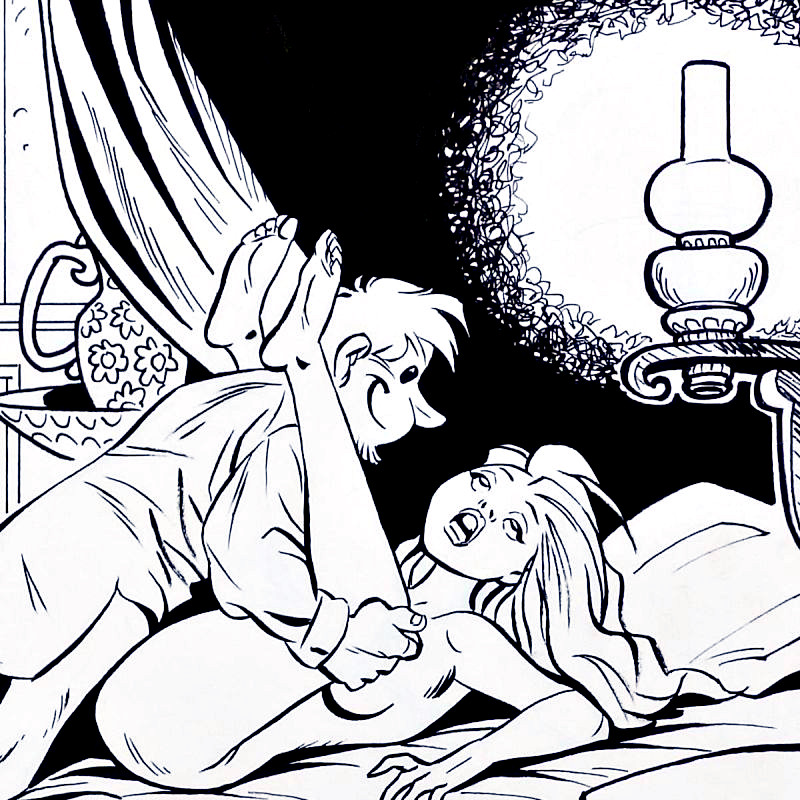
\includegraphics[width=0.6\textwidth]{images/en_revenant_de_paris.jpg}
\end{center}
%\\\\En m'asseyant, je vis son con
%\\Brindezingue, la faridondon
%\\Il était noir comm'du charbon
%
%\\\\Il était noir comm'du charbon
%\\Brindezingue, la faridondon
%\\Et tout couvert de morpi-ons
%\\\\Et tout couvert de morpi-ons
% \\Brindezingue, la faridondon
%\\Y en avait cinq cent millions
%\\\\Y en avait cinq cent millions
% \\Brindezingue, la faridondon
%\\Qui défilaient par escadrons
%\\\\Qui défilaient par escadrons
% \\Brindezingue, la faridondon
%\\Comm'les soldats d'Napoléon
%\\\\Comm'les soldats d'Napoléon
% \\Brindezingue, la faridondon
%\\Et moi, comme un foutu cochon
%\\\\Et moi, comme un foutu cochon
% \\Brindezingue, la faridondon
%\\J'ai baisé la Marie-Suzon

\breakpage